% Model Card do T2 (INF01017 - Aprendizado de Máquina, UFRGS), no formato de Mitchell et al. (2019), Figura 2.
% Compila com pdfLaTeX (padrão do Overleaf) ou XeLaTeX. As figuras ficam na pasta figuras/.
% Os trechos \pendente{...} marcam o que o grupo ainda precisa escrever.
\documentclass[10pt,a4paper]{article}
\usepackage{iftex}
\ifPDFTeX
  \usepackage[utf8]{inputenc}
  \usepackage[T1]{fontenc}
\fi
\usepackage[brazilian]{babel}
\usepackage{libertine}
\usepackage[a4paper,left=1.9cm,right=1.9cm,top=2.0cm,bottom=2.0cm,footskip=0.9cm]{geometry}
\usepackage{graphicx,booktabs,tabularx,array,makecell,enumitem,xcolor,paracol,eso-pic,tikz,tikzpagenodes,needspace,placeins}
\usepackage{xurl}
\usepackage[colorlinks=true,urlcolor=linkblue,linkcolor=linkblue]{hyperref}
\definecolor{linkblue}{HTML}{1155CC}
\urlstyle{same}
\definecolor{pendente}{HTML}{B4461B}
\graphicspath{{figuras/}}

% Moldura em todas as páginas, como no cartão do artigo
\AddToShipoutPictureBG{\begin{tikzpicture}[remember picture,overlay]
  \draw[black!60,line width=0.5pt] ([xshift=-9pt,yshift=-9pt]current page text area.south west)
    rectangle ([xshift=9pt,yshift=9pt]current page text area.north east);
\end{tikzpicture}}

\setlength{\parindent}{0pt}
\setlength{\parskip}{2pt}
\setlength{\emergencystretch}{2em}
\setlength{\columnsep}{14pt}
\setlist[itemize]{leftmargin=1.05em,label=\textbullet,topsep=1pt,itemsep=1.5pt,parsep=0pt}
\renewcommand{\arraystretch}{1.12}
\setlength{\tabcolsep}{4pt}
\setcellgapes{1pt}

% Título de seção do cartão (negrito, sem numeração) e subtítulo dentro da seção
% (\FloatBarrier mantém as figuras dentro da seção ou subseção em que aparecem)
\newcommand{\secao}[1]{\FloatBarrier\Needspace{4\baselineskip}\par\vspace{7pt}{\large\bfseries #1}\par\vspace{2pt}}
\newcommand{\subsecao}[2][4]{\FloatBarrier\Needspace{#1\baselineskip}\par\vspace{5pt}{\bfseries #2}\par\vspace{1pt}}
\setlength{\textfloatsep}{8pt plus 2pt minus 2pt}
\setlength{\floatsep}{8pt plus 2pt minus 2pt}
\setlength{\intextsep}{8pt plus 2pt minus 2pt}
\renewcommand{\topfraction}{0.9}
\renewcommand{\bottomfraction}{0.8}
\renewcommand{\textfraction}{0.07}
\renewcommand{\floatpagefraction}{0.8}
\makeatletter % páginas só de figuras começam no topo, sem centralizar verticalmente
\setlength{\@fptop}{0pt}
\setlength{\@fpsep}{10pt plus 2pt}
\setlength{\@fpbot}{0pt plus 1fil}
\makeatother
% Marcador do que o grupo ainda precisa escrever
\newcommand{\pendente}[1]{{\color{pendente}\itshape[A definir pelo grupo: #1]}}
\newcommand{\legenda}[1]{\par\vspace{1pt}{\centering\small\itshape #1\par}\vspace{4pt}}

\begin{document}
\shorthandoff{"}

\begin{center}
{\LARGE\bfseries Model Card - Detector de Ataques Cardíacos}\par\vspace{4pt}
{\small Grupo: Gabriel Pieruccini Knopp (cartão 00594975) e Vítor Santana Feijó (cartão 00588403)}\par
{\small INF01017 - Aprendizado de Máquina, Instituto de Informática, UFRGS\enspace$\cdot$\enspace Repositório: \url{https://github.com/vitorsfeijo/Trabalho_ML}}
\end{center}
\vspace{2pt}

\columnratio{0.6}
\begin{paracol}{2}

\secao{Model Details}
\begin{itemize}
\item Desenvolvido por Gabriel Pieruccini Knopp e Vítor Santana Feijó na disciplina INF01017 - Aprendizado de Máquina (Instituto de Informática, UFRGS), novembro de 2026, versão 1.0 (primeira versão; continuação do spot-checking do T1).
\item Regressão Logística (C = 0,1; penalidade L2) com limiar de decisão 0,45, em um Pipeline do scikit-learn: imputação pela mediana, padronização z-score dos atributos numéricos e one-hot encoding dos nominais (13 atributos clínicos, 22 colunas de entrada).
\item Escolhida pelo grupo entre os três algoritmos indicados pelo T1 (Regressão Logística, KNN e Random Forest), com base no desempenho no conjunto de teste. Os três foram otimizados com nested cross-validation estratificada (5 folds externos $\times$ 3 internos): Grid Search para a Regressão Logística e o KNN e Optuna (50 trials) para o Random Forest, com o limiar de decisão otimizado como mais um hiperparâmetro. Nenhuma restrição de fairness foi aplicada.
\item Features: age, sex, cp, trestbps, chol, fbs, restecg, thalach, exang, oldpeak, slope, ca e thal.
\item Código, notebooks e figuras de resultados (pasta figuras/): no repositório indicado no cabeçalho.
\item \pendente{forma de citação, licença de uso e canal de contato}
\end{itemize}

\secao{Intended Use}
\begin{itemize}
\item \textbf{Usos primários:} \pendente{tarefas e contextos para os quais o modelo foi desenvolvido}
\item \textbf{Usuários primários:} \pendente{perfil de quem se espera que use o modelo}
\item \textbf{Fora do escopo:} \pendente{usos que o modelo pode parecer cobrir, mas para os quais não foi projetado}
\end{itemize}

\secao{Factors}
\begin{itemize}
\item \textbf{Fatores relevantes:} \pendente{fatores previsivelmente relevantes para o desempenho e como foram identificados}
\item \textbf{Fatores de avaliação:} sexo (feminino e masculino), faixa etária ($<$ 55 e $\geq$ 55 anos; 55 é a mediana de idade do treino) e a interseção sexo $\times$ faixa etária. A base não tem fatores de instrumentação ou de ambiente que variem entre os pacientes.
\item \pendente{por que esses fatores foram escolhidos e implicações dos fatores relevantes não avaliados}
\end{itemize}

\secao{Metrics}
\begin{itemize}
\item Métrica principal: \textbf{F1-score} da classe positiva (com doença), a mesma do T1. Também são reportadas acurácia, precisão, recall, ROC-AUC e PR-AUC.
\item Por grupo, além do F1: \textbf{taxa de falsos positivos} (TFP), \textbf{taxa de falsos negativos} (TFN), \textbf{taxa de falsa descoberta} (TFD) e \textbf{taxa de falsa omissão} (TFO), obtidas da matriz de confusão. Paridade de TFN entre grupos corresponde à Igualdade de Oportunidade; paridade de TFN e TFP, à Igualdade de Chances.
\item Limiar de decisão otimizado na CV interna junto com os hiperparâmetros: limiares de 0,10 a 0,90 (passo 0,05), escolhendo o de maior F1 médio nos folds internos (empates: o mais próximo de 0,5). Limiar final: 0,45.
\item \pendente{efeito do limiar e custos de cada tipo de erro no contexto do problema}
\item Incerteza: média e desvio padrão nos 5 folds externos da nested CV; IC 95\% por bootstrap (1000 reamostragens dentro de cada grupo) nas métricas por grupo. Com 61 pacientes no teste, um único paciente classificado de outra forma altera o F1 em 2 a 3 pontos.
\end{itemize}

\secao{Training Data}
\begin{itemize}
\item Base Cleveland do UCI Heart Disease (Janosi et al., 1988), com pacientes da Cleveland Clinic Foundation (EUA) avaliados para doença arterial coronariana, na versão do Kaggle ``Health care: Data set on Heart attack possibility'' (Bhat). Base escolhida pelo grupo no T1.
\item Dos 303 registros, 1 duplicata foi removida (302 pacientes); nenhum atributo foi removido. Treino: 241 pacientes (80\%), 110 com doença (45,6\%).
\item Pré-processamento: alvo recodificado para 1 = com doença (o target do Kaggle tem o sentido invertido em relação à UCI); códigos de ausência (ca = 4 e thal = 0) marcados como ausentes e imputados pela mediana; z-score nos numéricos; one-hot nos nominais (cp, restecg, slope e thal). Tudo em um Pipeline ajustado só nos dados de treino.
\item Pacientes (com doença) por grupo:\par\vspace{2pt}
{\footnotesize \begin{tabular}{@{}l c c@{}}
\toprule
Grupo & Treino & Teste \\
\midrule
Todos & 241 (110) & 61 (28) \\
Feminino & 79 (20) & 17 (4) \\
Masculino & 162 (90) & 44 (24) \\
$<$ 55 & 114 (36) & 29 (8) \\
$\geq$ 55 & 127 (74) & 32 (20) \\
Feminino, $<$ 55 & 33 (2) & 7 (0) \\
Feminino, $\geq$ 55 & 46 (18) & 10 (4) \\
Masculino, $<$ 55 & 81 (34) & 22 (8) \\
Masculino, $\geq$ 55 & 81 (56) & 22 (16) \\
\bottomrule
\end{tabular}}
\item Limitações conhecidas: base pequena, coletada em uma única instituição; o Kaggle documenta thal e o alvo de forma diferente da base original. \pendente{como essas limitações podem ter introduzido vieses no modelo}
\end{itemize}

\switchcolumn

\secao{Quantitative Analyses}
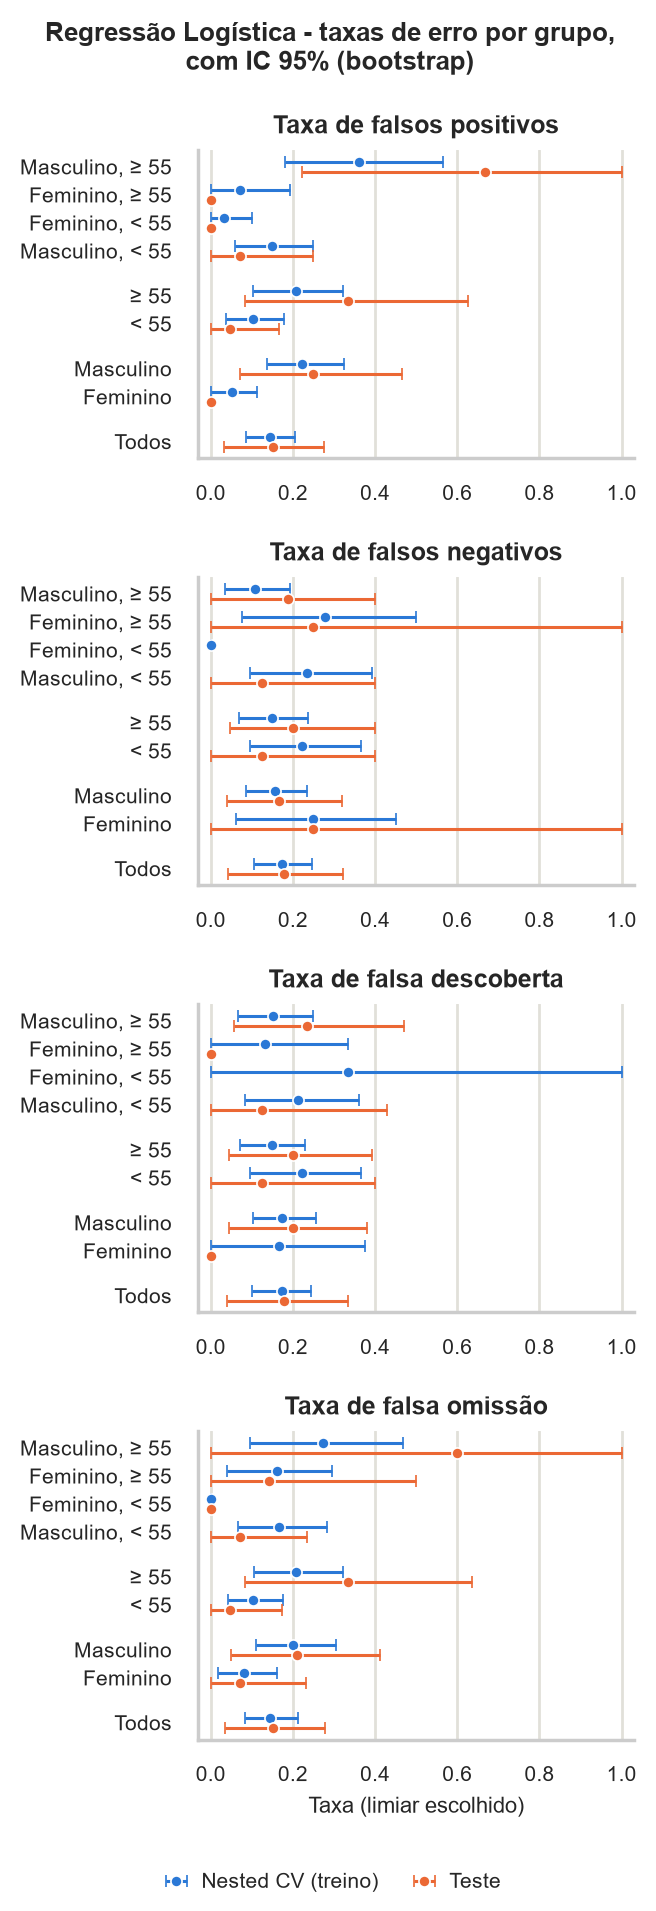
\includegraphics[width=\linewidth]{t2_taxas.png}
{\footnotesize Pontos: valor da taxa; barras: IC 95\% (bootstrap). Azul: predições fora da amostra da nested CV (241 pacientes de treino); laranja: modelo final no teste (61 pacientes). Taxas indefinidas (por exemplo, TFN em grupo sem pacientes com doença) não aparecem. Tabelas na continuação desta seção.\par}

\secao{Evaluation Data}
\begin{itemize}
\item Conjunto de teste com 61 pacientes (20\% da base, amostragem estratificada com random\_state = 42, reservado desde o T1): 28 com doença e 33 sem. Ele não foi usado em nenhuma etapa de seleção de hiperparâmetros ou de modelos.
\item Também são reportadas as predições fora da amostra da nested CV: cada um dos 241 pacientes de treino é previsto por um modelo que não o viu, com o limiar escolhido no seu fold.
\item Motivação: amostra aleatória estratificada da mesma base, para estimar o desempenho em dados nunca vistos. Não há conjunto de avaliação externo (de outra instituição ou período) disponível.
\item Pré-processamento: o mesmo pipeline do treino, com parâmetros (medianas, médias, desvios e categorias) aprendidos apenas nos dados de treino.
\end{itemize}
\end{paracol}

\secao{Quantitative Analyses (continuação)}

\subsecao[12]{Otimização e seleção do modelo}
{\footnotesize \begin{tabularx}{\linewidth}{@{}>{\raggedright\arraybackslash}p{2.3cm} >{\raggedright\arraybackslash}p{2.2cm} >{\raggedright\arraybackslash}X >{\raggedright\arraybackslash}p{4.3cm} c@{}}
\toprule
Algoritmo & Busca & Espaço de busca & Configuração final & Limiar \\
\midrule
Regressão Logística & Grid Search (12 configurações) & C $\in$ \{0,001; 0,01; 0,1; 1; 10; 100\}; penalidade L1 ou L2 & C = 0,1; penalidade L2 & 0,45 \\
\addlinespace[2pt]
KNN & Grid Search (160 configurações) & k de 1 a 40; distância Manhattan ou Euclidiana; pesos uniformes ou pela distância & k = 9; distância Manhattan; pesos pela distância & 0,45 \\
\addlinespace[2pt]
Random Forest & Optuna (TPE, 50 trials) & n\_estimators de 100 a 500 (passo 50); max\_depth sem limite ou de 2 a 15; min\_samples\_leaf de 1 a 10; max\_features $\in$ \{sqrt; log2; 0,5\} & 150 árvores; max\_depth = sem limite; min\_samples\_leaf = 5; max\_features = log2 & 0,50 \\
\bottomrule
\end{tabularx}}
\vspace{6pt}

{\footnotesize \begin{tabularx}{\linewidth}{@{}l l *{6}{>{\centering\arraybackslash}X}@{}}
\toprule
Algoritmo & Dados & F1 & Acurácia & Precisão & Recall & ROC-AUC & PR-AUC \\
\midrule
Regressão Logística & Nested CV & 0,827 (0,058) & 0,842 (0,053) & 0,832 (0,076) & 0,827 (0,081) & 0,902 (0,048) & 0,901 (0,051) \\
 & Teste & \textbf{0,821} & 0,836 & 0,821 & 0,821 & 0,922 & 0,909 \\ \addlinespace[2pt]
KNN & Nested CV & 0,811 (0,040) & 0,822 (0,047) & 0,803 (0,099) & 0,836 (0,094) & 0,903 (0,037) & 0,910 (0,026) \\
 & Teste & \textbf{0,800} & 0,820 & 0,815 & 0,786 & 0,893 & 0,852 \\ \addlinespace[2pt]
Random Forest & Nested CV & 0,808 (0,039) & 0,818 (0,054) & 0,806 (0,117) & 0,827 (0,081) & 0,916 (0,032) & 0,920 (0,028) \\
 & Teste & \textbf{0,755} & 0,787 & 0,800 & 0,714 & 0,883 & 0,868 \\ \addlinespace[2pt]
\bottomrule
\end{tabularx}}
\legenda{Nested CV: média (desvio padrão) nos 5 folds externos. Teste: modelo final de cada algoritmo, avaliado uma única vez.}
\begin{itemize}
\item F1 no teste com o limiar padrão de 0,5, para referência: Regressão Logística: 0,830; KNN: 0,815; Random Forest: 0,755.
\item Hiperparâmetros que mudaram entre os 5 folds externos: Regressão Logística: limiar, C, penalidade; KNN: limiar, k, pesos; Random Forest: limiar, n\_estimators, max\_depth, min\_samples\_leaf, max\_features.
\end{itemize}
\begin{figure}[!htbp]\centering
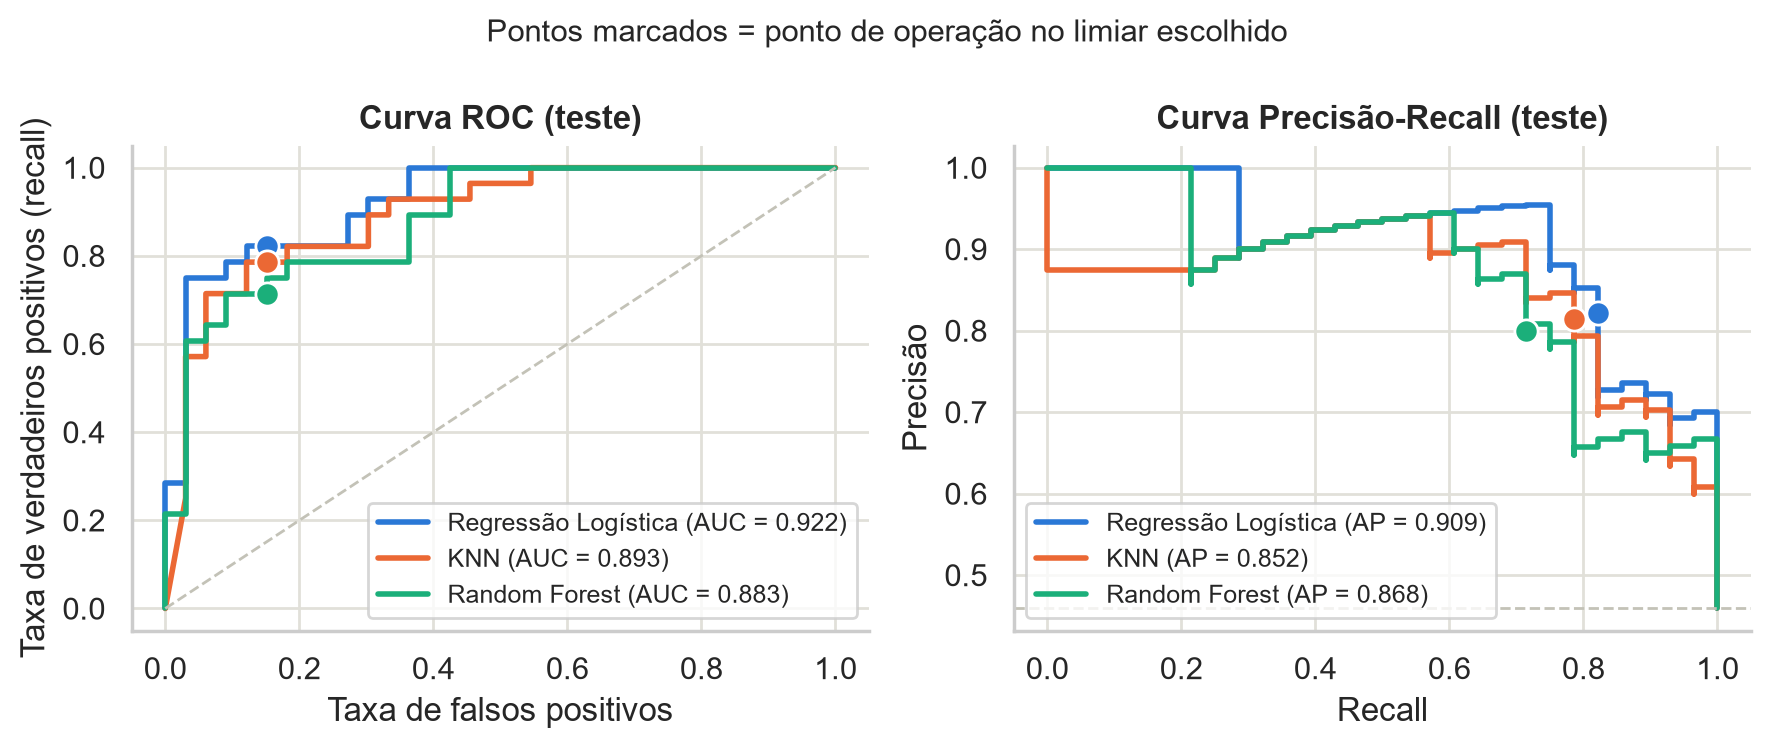
\includegraphics[width=0.86\linewidth]{t2_roc_pr.png}
\legenda{Curvas ROC e Precisão-Recall no teste; pontos marcados = ponto de operação de cada modelo no limiar escolhido.}
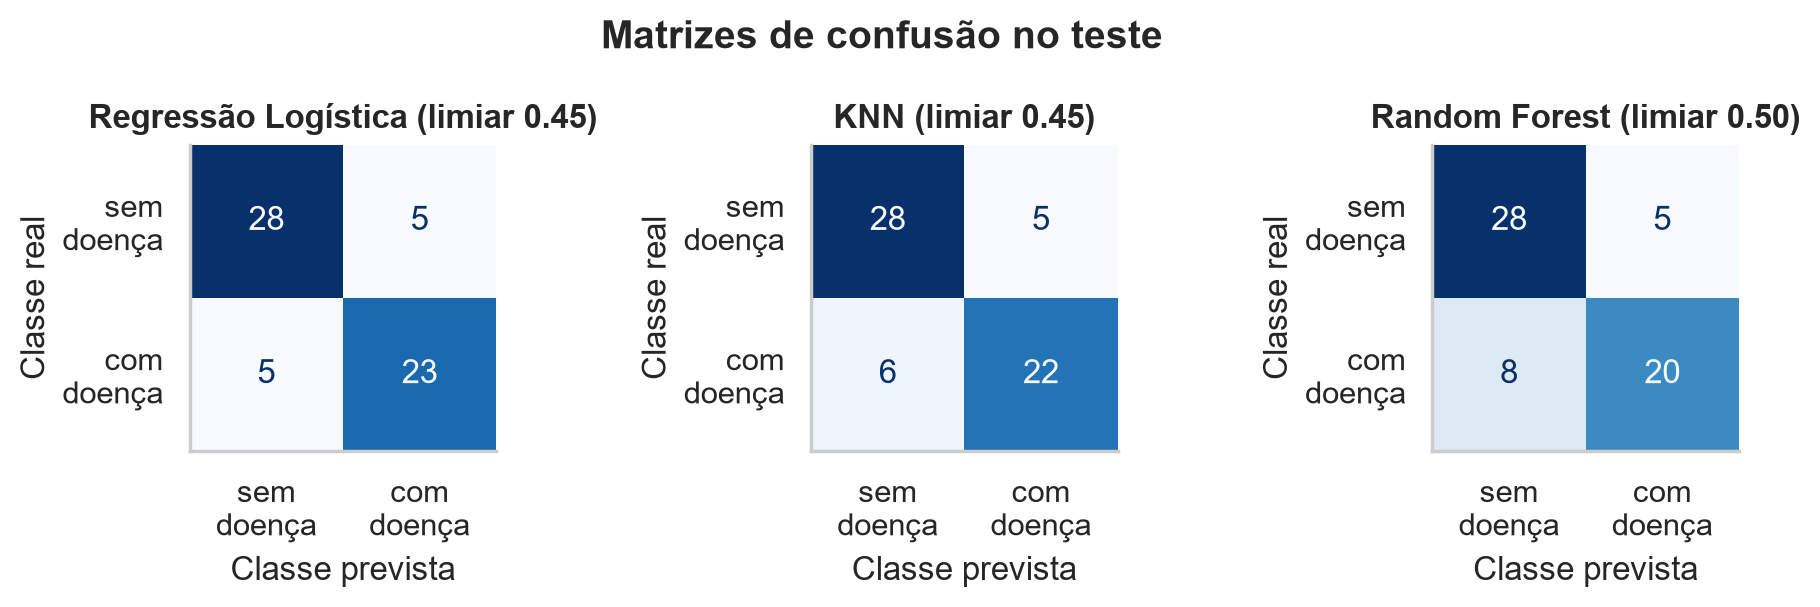
\includegraphics[width=0.92\linewidth]{t2_confusao.png}
\legenda{Matrizes de confusão no teste, no limiar escolhido de cada modelo.}
\end{figure}
\begin{itemize}
\item \pendente{comparação dos modelos: pontos fortes e fracos de cada um e justificativa da escolha da Regressão Logística}
\end{itemize}

\subsecao[24]{Resultados unitários (Regressão Logística)}
{\footnotesize \begin{tabularx}{\linewidth}{@{}l l c *{5}{>{\centering\arraybackslash}X}@{}}
\toprule
Grupo & Dados & n (com doença) & F1 & TFP & TFN & TFD & TFO \\
\midrule
Todos & Nested CV & 241 (110) & \makecell{0,83\\[-1pt]{\scriptsize [0,77; 0,88]}} & \makecell{0,15\\[-1pt]{\scriptsize [0,09; 0,21]}} & \makecell{0,17\\[-1pt]{\scriptsize [0,10; 0,25]}} & \makecell{0,17\\[-1pt]{\scriptsize [0,10; 0,24]}} & \makecell{0,15\\[-1pt]{\scriptsize [0,08; 0,21]}} \\
 & Teste & 61 (28) & \makecell{0,82\\[-1pt]{\scriptsize [0,70; 0,92]}} & \makecell{0,15\\[-1pt]{\scriptsize [0,03; 0,28]}} & \makecell{0,18\\[-1pt]{\scriptsize [0,04; 0,32]}} & \makecell{0,18\\[-1pt]{\scriptsize [0,04; 0,33]}} & \makecell{0,15\\[-1pt]{\scriptsize [0,03; 0,28]}} \\ \addlinespace[2pt]
Feminino & Nested CV & 79 (20) & \makecell{0,79\\[-1pt]{\scriptsize [0,61; 0,91]}} & \makecell{0,05\\[-1pt]{\scriptsize [0,00; 0,11]}} & \makecell{0,25\\[-1pt]{\scriptsize [0,06; 0,45]}} & \makecell{0,17\\[-1pt]{\scriptsize [0,00; 0,38]}} & \makecell{0,08\\[-1pt]{\scriptsize [0,02; 0,16]}} \\
 & Teste & 17 (4) & \makecell{0,86\\[-1pt]{\scriptsize [0,00; 1,00]}} & \makecell{0,00\\[-1pt]{\scriptsize [0,00; 0,00]}} & \makecell{0,25\\[-1pt]{\scriptsize [0,00; 1,00]}} & \makecell{0,00\\[-1pt]{\scriptsize [0,00; 0,00]}} & \makecell{0,07\\[-1pt]{\scriptsize [0,00; 0,23]}} \\ \addlinespace[2pt]
Masculino & Nested CV & 162 (90) & \makecell{0,84\\[-1pt]{\scriptsize [0,77; 0,89]}} & \makecell{0,22\\[-1pt]{\scriptsize [0,14; 0,32]}} & \makecell{0,16\\[-1pt]{\scriptsize [0,09; 0,23]}} & \makecell{0,17\\[-1pt]{\scriptsize [0,10; 0,26]}} & \makecell{0,20\\[-1pt]{\scriptsize [0,11; 0,31]}} \\
 & Teste & 44 (24) & \makecell{0,82\\[-1pt]{\scriptsize [0,68; 0,92]}} & \makecell{0,25\\[-1pt]{\scriptsize [0,07; 0,47]}} & \makecell{0,17\\[-1pt]{\scriptsize [0,04; 0,32]}} & \makecell{0,20\\[-1pt]{\scriptsize [0,04; 0,38]}} & \makecell{0,21\\[-1pt]{\scriptsize [0,05; 0,41]}} \\ \addlinespace[2pt]
$<$ 55 & Nested CV & 114 (36) & \makecell{0,78\\[-1pt]{\scriptsize [0,66; 0,87]}} & \makecell{0,10\\[-1pt]{\scriptsize [0,04; 0,18]}} & \makecell{0,22\\[-1pt]{\scriptsize [0,10; 0,37]}} & \makecell{0,22\\[-1pt]{\scriptsize [0,10; 0,37]}} & \makecell{0,10\\[-1pt]{\scriptsize [0,04; 0,18]}} \\
 & Teste & 29 (8) & \makecell{0,88\\[-1pt]{\scriptsize [0,67; 1,00]}} & \makecell{0,05\\[-1pt]{\scriptsize [0,00; 0,17]}} & \makecell{0,12\\[-1pt]{\scriptsize [0,00; 0,40]}} & \makecell{0,12\\[-1pt]{\scriptsize [0,00; 0,40]}} & \makecell{0,05\\[-1pt]{\scriptsize [0,00; 0,17]}} \\ \addlinespace[2pt]
$\geq$ 55 & Nested CV & 127 (74) & \makecell{0,85\\[-1pt]{\scriptsize [0,79; 0,91]}} & \makecell{0,21\\[-1pt]{\scriptsize [0,10; 0,32]}} & \makecell{0,15\\[-1pt]{\scriptsize [0,07; 0,24]}} & \makecell{0,15\\[-1pt]{\scriptsize [0,07; 0,23]}} & \makecell{0,21\\[-1pt]{\scriptsize [0,11; 0,32]}} \\
 & Teste & 32 (20) & \makecell{0,80\\[-1pt]{\scriptsize [0,63; 0,92]}} & \makecell{0,33\\[-1pt]{\scriptsize [0,08; 0,62]}} & \makecell{0,20\\[-1pt]{\scriptsize [0,05; 0,40]}} & \makecell{0,20\\[-1pt]{\scriptsize [0,05; 0,39]}} & \makecell{0,33\\[-1pt]{\scriptsize [0,08; 0,64]}} \\ \addlinespace[2pt]
\bottomrule
\end{tabularx}}
\legenda{Valor e IC 95\% por bootstrap (1000 reamostragens dentro de cada grupo). Nested CV: predições fora da amostra dos 241 pacientes de treino; Teste: modelo final nos 61 pacientes de teste. indef.: métrica indefinida no grupo.}
\begin{itemize}
\item \pendente{discussão do desempenho por sexo e por faixa etária}
\end{itemize}

\subsecao[20]{Resultados interseccionais (Regressão Logística)}
{\footnotesize \begin{tabularx}{\linewidth}{@{}l l c *{5}{>{\centering\arraybackslash}X}@{}}
\toprule
Grupo & Dados & n (com doença) & F1 & TFP & TFN & TFD & TFO \\
\midrule
Feminino, $<$ 55 & Nested CV & 33 (2) & \makecell{0,80\\[-1pt]{\scriptsize [0,40; 1,00]}} & \makecell{0,03\\[-1pt]{\scriptsize [0,00; 0,10]}} & \makecell{0,00\\[-1pt]{\scriptsize [0,00; 0,00]}} & \makecell{0,33\\[-1pt]{\scriptsize [0,00; 1,00]}} & \makecell{0,00\\[-1pt]{\scriptsize [0,00; 0,00]}} \\
 & Teste & 7 (0) & \textit{indef.} & \makecell{0,00\\[-1pt]{\scriptsize [0,00; 0,00]}} & \textit{indef.} & \textit{indef.} & \makecell{0,00\\[-1pt]{\scriptsize [0,00; 0,00]}} \\ \addlinespace[2pt]
Feminino, $\geq$ 55 & Nested CV & 46 (18) & \makecell{0,79\\[-1pt]{\scriptsize [0,61; 0,92]}} & \makecell{0,07\\[-1pt]{\scriptsize [0,00; 0,19]}} & \makecell{0,28\\[-1pt]{\scriptsize [0,08; 0,50]}} & \makecell{0,13\\[-1pt]{\scriptsize [0,00; 0,33]}} & \makecell{0,16\\[-1pt]{\scriptsize [0,04; 0,30]}} \\
 & Teste & 10 (4) & \makecell{0,86\\[-1pt]{\scriptsize [0,00; 1,00]}} & \makecell{0,00\\[-1pt]{\scriptsize [0,00; 0,00]}} & \makecell{0,25\\[-1pt]{\scriptsize [0,00; 1,00]}} & \makecell{0,00\\[-1pt]{\scriptsize [0,00; 0,00]}} & \makecell{0,14\\[-1pt]{\scriptsize [0,00; 0,50]}} \\ \addlinespace[2pt]
Masculino, $<$ 55 & Nested CV & 81 (34) & \makecell{0,78\\[-1pt]{\scriptsize [0,65; 0,88]}} & \makecell{0,15\\[-1pt]{\scriptsize [0,06; 0,25]}} & \makecell{0,24\\[-1pt]{\scriptsize [0,10; 0,39]}} & \makecell{0,21\\[-1pt]{\scriptsize [0,08; 0,36]}} & \makecell{0,17\\[-1pt]{\scriptsize [0,07; 0,28]}} \\
 & Teste & 22 (8) & \makecell{0,88\\[-1pt]{\scriptsize [0,62; 1,00]}} & \makecell{0,07\\[-1pt]{\scriptsize [0,00; 0,25]}} & \makecell{0,12\\[-1pt]{\scriptsize [0,00; 0,40]}} & \makecell{0,12\\[-1pt]{\scriptsize [0,00; 0,43]}} & \makecell{0,07\\[-1pt]{\scriptsize [0,00; 0,24]}} \\ \addlinespace[2pt]
Masculino, $\geq$ 55 & Nested CV & 81 (56) & \makecell{0,87\\[-1pt]{\scriptsize [0,80; 0,93]}} & \makecell{0,36\\[-1pt]{\scriptsize [0,18; 0,57]}} & \makecell{0,11\\[-1pt]{\scriptsize [0,03; 0,19]}} & \makecell{0,15\\[-1pt]{\scriptsize [0,07; 0,25]}} & \makecell{0,27\\[-1pt]{\scriptsize [0,10; 0,47]}} \\
 & Teste & 22 (16) & \makecell{0,79\\[-1pt]{\scriptsize [0,61; 0,92]}} & \makecell{0,67\\[-1pt]{\scriptsize [0,22; 1,00]}} & \makecell{0,19\\[-1pt]{\scriptsize [0,00; 0,40]}} & \makecell{0,24\\[-1pt]{\scriptsize [0,06; 0,47]}} & \makecell{0,60\\[-1pt]{\scriptsize [0,00; 1,00]}} \\ \addlinespace[2pt]
\bottomrule
\end{tabularx}}
\legenda{Mesmo formato da tabela anterior. No teste, os subgrupos têm de 7 a 22 pacientes.}
\begin{itemize}
\item \pendente{discussão dos resultados interseccionais e da paridade entre grupos (Igualdade de Oportunidade e Igualdade de Chances)}
\end{itemize}

\subsecao[10]{Análise de erros (Regressão Logística)}
{\footnotesize \begin{tabularx}{\linewidth}{@{}l c c c c >{\centering\arraybackslash}X c c c >{\centering\arraybackslash}X@{}}
\toprule
 & & \multicolumn{4}{c}{Pacientes com doença} & \multicolumn{4}{c}{Pacientes sem doença} \\
\cmidrule(lr){3-6}\cmidrule(l){7-10}
Dados & Pacientes & n & FN & TFN & FN com prob. $<$ 0,25 & n & FP & TFP & FP com prob. $>$ 0,75 \\
\midrule
Nested CV (treino) & 241 & 110 & 19 & 0,173 & 7 & 131 & 19 & 0,145 & 4 \\
Teste & 61 & 28 & 5 & 0,179 & 1 & 33 & 5 & 0,152 & 1 \\
\bottomrule
\end{tabularx}}
\legenda{FN e FP com alta confiança: erros com probabilidade prevista de doença abaixo de 0,25 (FN) ou acima de 0,75 (FP).}
\begin{figure}[!htbp]\centering
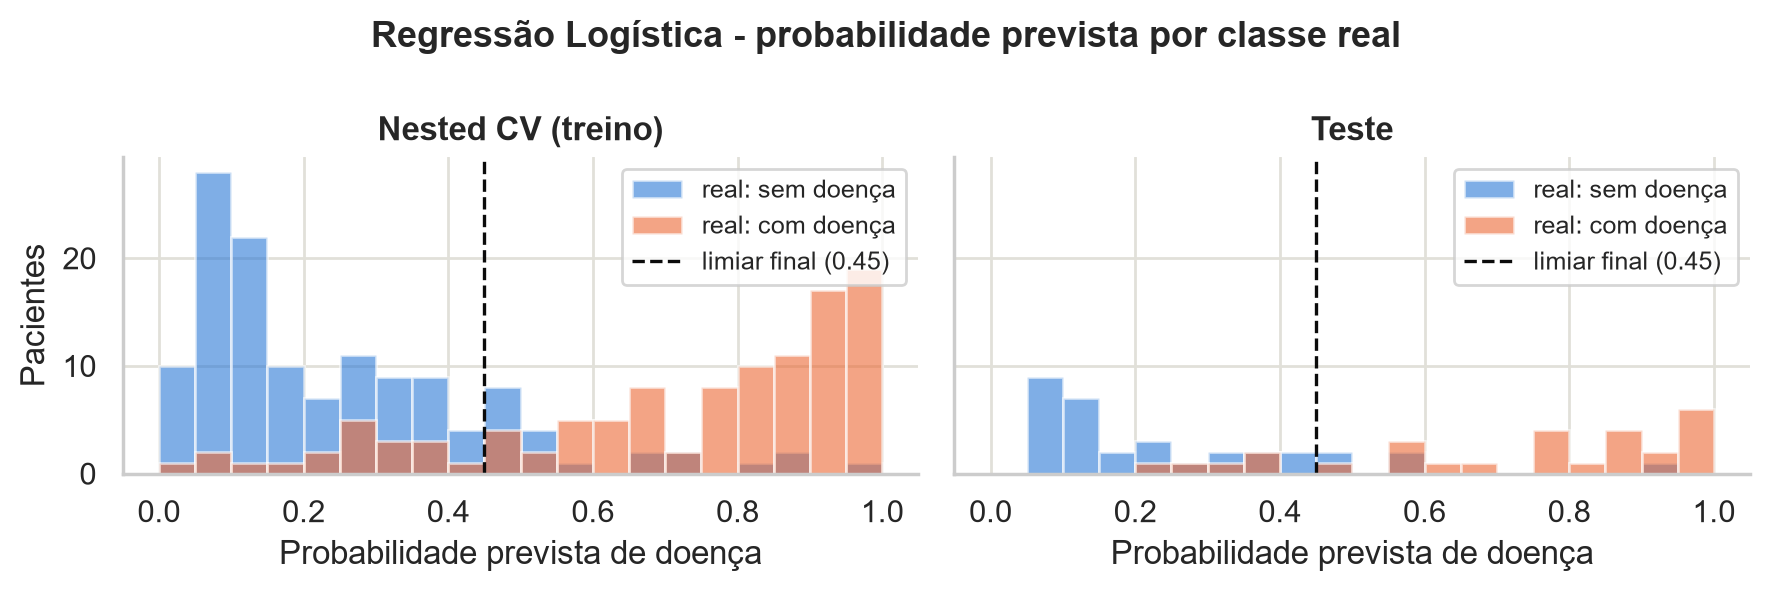
\includegraphics[width=0.9\linewidth]{t2_probabilidades.png}
\legenda{Probabilidade prevista de doença por classe real; a linha tracejada é o limiar final.}
\end{figure}
{\footnotesize \begin{tabularx}{\linewidth}{@{}X *{4}{c}@{}}
\toprule
Atributo (média ou \%) & VP (n=114) & FN (n=24) & VN (n=140) & FP (n=24) \\
\midrule
age (anos) & 57,0 & 54,9 & 51,8 & 57,2 \\
trestbps (mm Hg) & 134,9 & 132,0 & 128,5 & 133,7 \\
chol (mg/dl) & 251,9 & 247,2 & 241,0 & 252,2 \\
thalach (bpm) & 135,7 & 155,4 & 160,0 & 148,8 \\
oldpeak & 1,8 & 0,7 & 0,5 & 1,1 \\
homens (\%) & 84,2 & 75,0 & 50,7 & 87,5 \\
dor assintomática, cp = 0 (\%) & 83,3 & 37,5 & 20,0 & 45,8 \\
angina no exercício, exang = 1 (\%) & 62,3 & 20,8 & 10,0 & 37,5 \\
ca $\geq$ 1 vaso (\%) & 74,6 & 29,2 & 15,7 & 37,5 \\
thal normal, thal = 2 (\%) & 16,7 & 70,8 & 86,4 & 33,3 \\
\bottomrule
\end{tabularx}}
\legenda{Perfil dos acertos e dos erros: média dos atributos numéricos e proporção de algumas categorias em cada tipo de resultado (nested CV e teste juntos, 302 pacientes).}
\begin{itemize}
\item \pendente{qual classe é mais difícil para o modelo e se há amostras ``confusas'', cujos atributos se parecem com os da outra classe}
\end{itemize}

\subsecao{Interpretabilidade (Regressão Logística)}
\begin{itemize}
\item Importância global: permutation importance no teste (queda do F1, limiar 0,45, ao embaralhar cada atributo original; 30 repetições) e SHAP (LinearExplainer, treino como referência) no teste, agregado por atributo original.
\item Coeficientes convertidos em medidas de efeito: odds ratio $e^{\beta}$ e efeito padronizado $\beta \cdot$ DP (variação do log-odds por 1 desvio padrão da coluna, o que deixa colunas de escalas diferentes comparáveis).
\item Partial dependence dos atributos numéricos.
\end{itemize}
\begin{figure}[!htbp]\centering
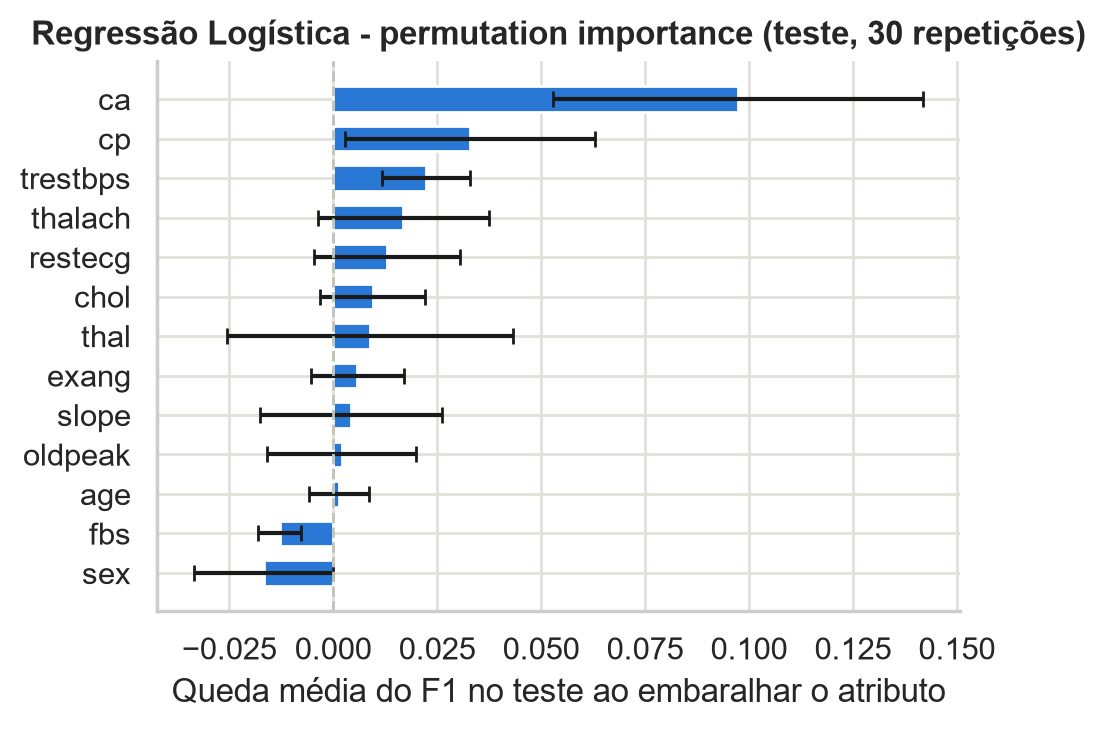
\includegraphics[width=0.49\linewidth]{t2_permutacao.png}\hfill
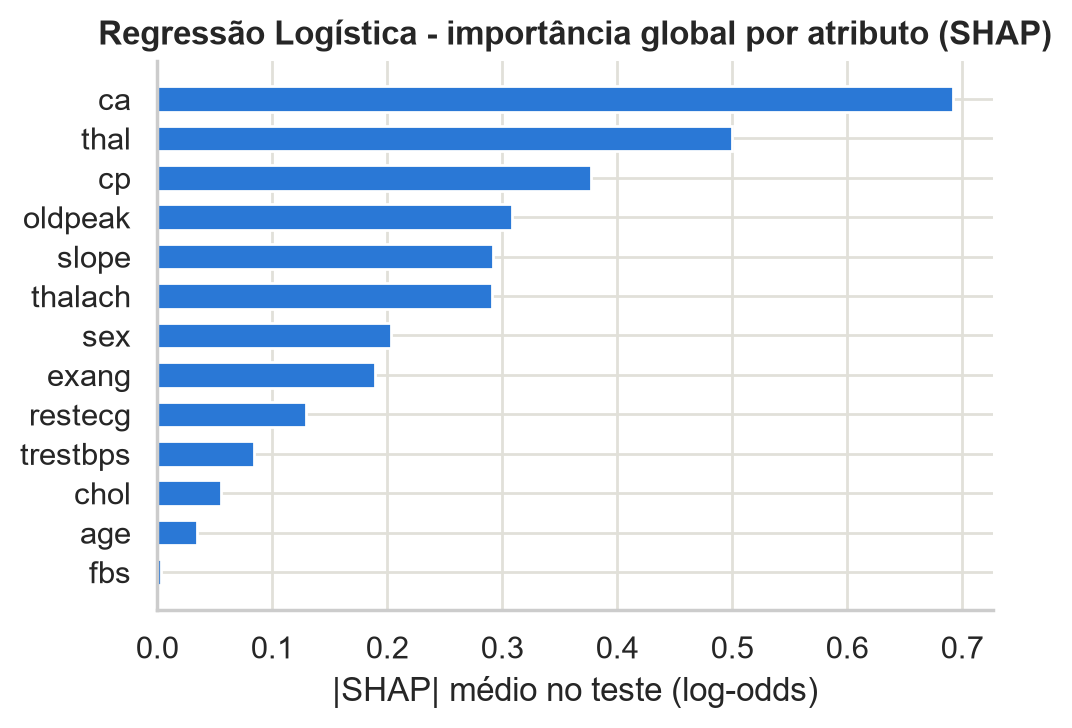
\includegraphics[width=0.49\linewidth]{t2_shap.png}
\legenda{Esquerda: permutation importance no teste (queda média do F1, com desvio padrão). Direita: importância global por atributo original via SHAP (média de |SHAP| no teste).}
\end{figure}
\begin{figure}[!htbp]\centering
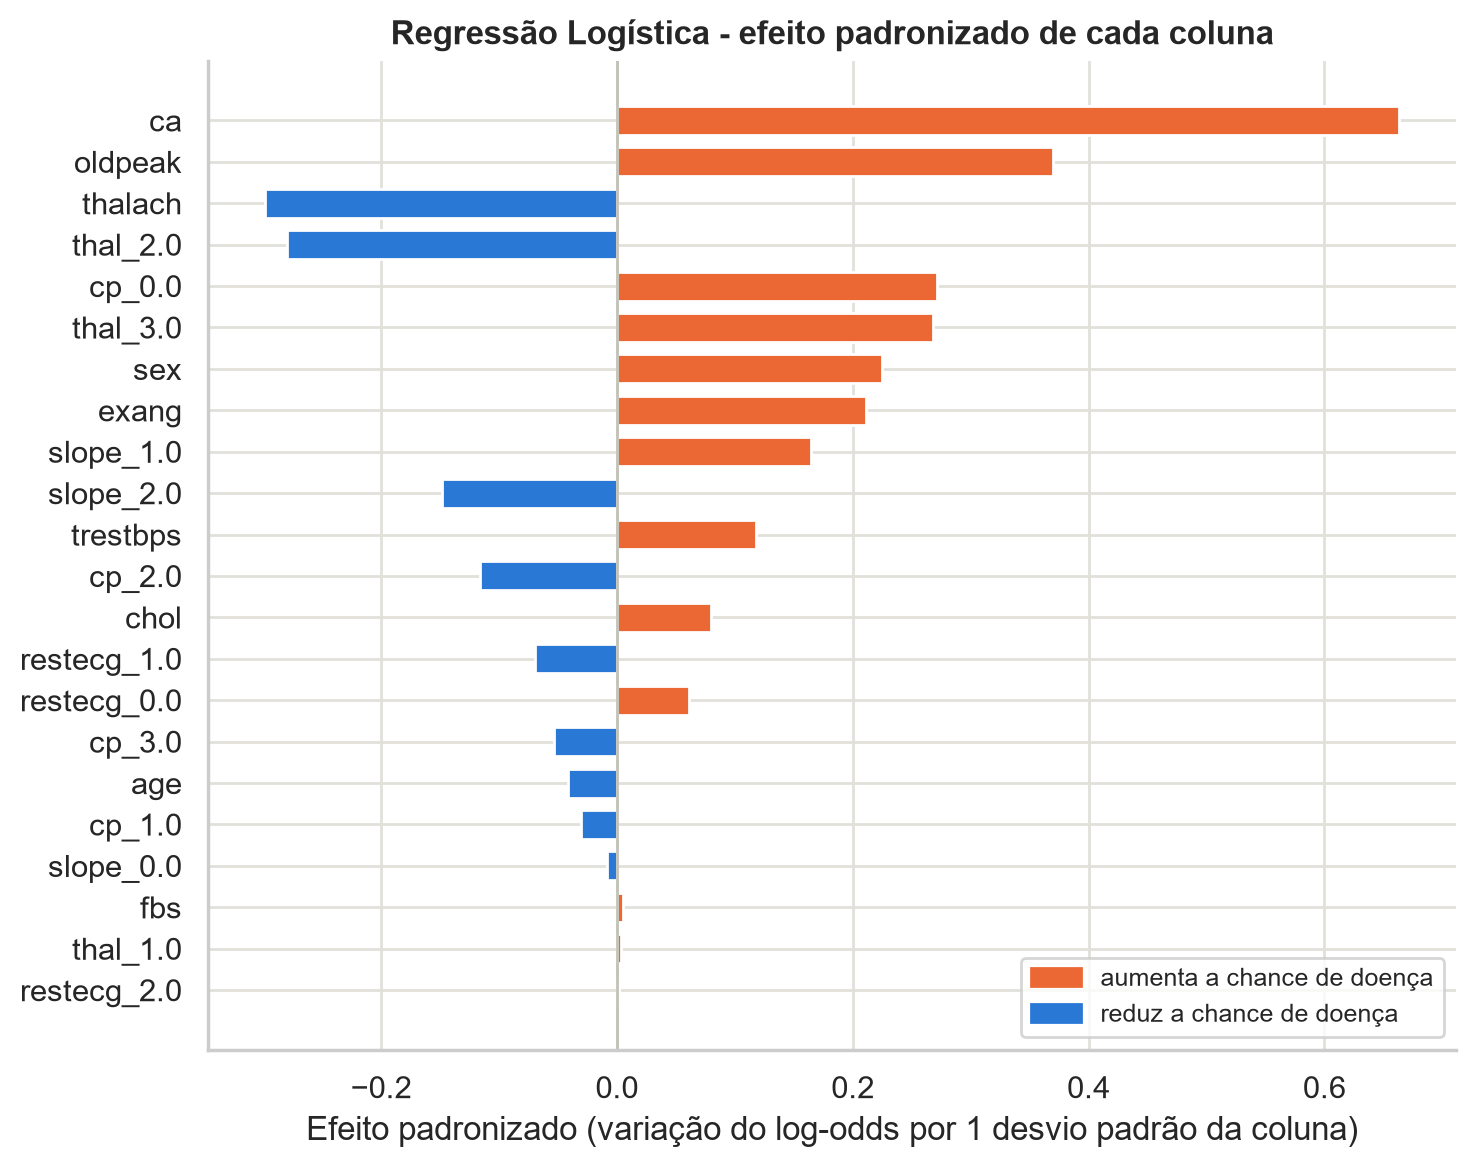
\includegraphics[width=0.7\linewidth]{t2_efeito.png}
\legenda{Efeito padronizado de cada coluna (laranja: aumenta a chance de doença; azul: reduz).}
{\footnotesize \begin{tabular}{@{}l l c c c@{}}
\toprule
Coluna & Unidade de $\beta$ & $\beta$ (log-odds) & Odds ratio $e^{\beta}$ & Efeito padronizado $\beta \cdot$ DP \\
\midrule
ca & +1 DP (0,9 vasos) & 0,664 & 1,942 & 0,664 \\
oldpeak & +1 DP (1,2) & 0,369 & 1,447 & 0,369 \\
thalach & +1 DP (21,9 bpm) & -0,298 & 0,742 & -0,298 \\
thal\_2.0 & presença (0 $\rightarrow$ 1) & -0,563 & 0,569 & -0,280 \\
cp\_0.0 & presença (0 $\rightarrow$ 1) & 0,543 & 1,720 & 0,271 \\
thal\_3.0 & presença (0 $\rightarrow$ 1) & 0,548 & 1,730 & 0,268 \\
sex & presença (0 $\rightarrow$ 1) & 0,480 & 1,615 & 0,225 \\
exang & presença (0 $\rightarrow$ 1) & 0,445 & 1,560 & 0,211 \\
slope\_1.0 & presença (0 $\rightarrow$ 1) & 0,330 & 1,391 & 0,165 \\
slope\_2.0 & presença (0 $\rightarrow$ 1) & -0,298 & 0,742 & -0,149 \\
\bottomrule
\end{tabular}}
\legenda{As 10 colunas de maior efeito padronizado em módulo. Nas colunas binárias e one-hot, a unidade é a presença da característica.}
\end{figure}
\begin{figure}[!htbp]\centering
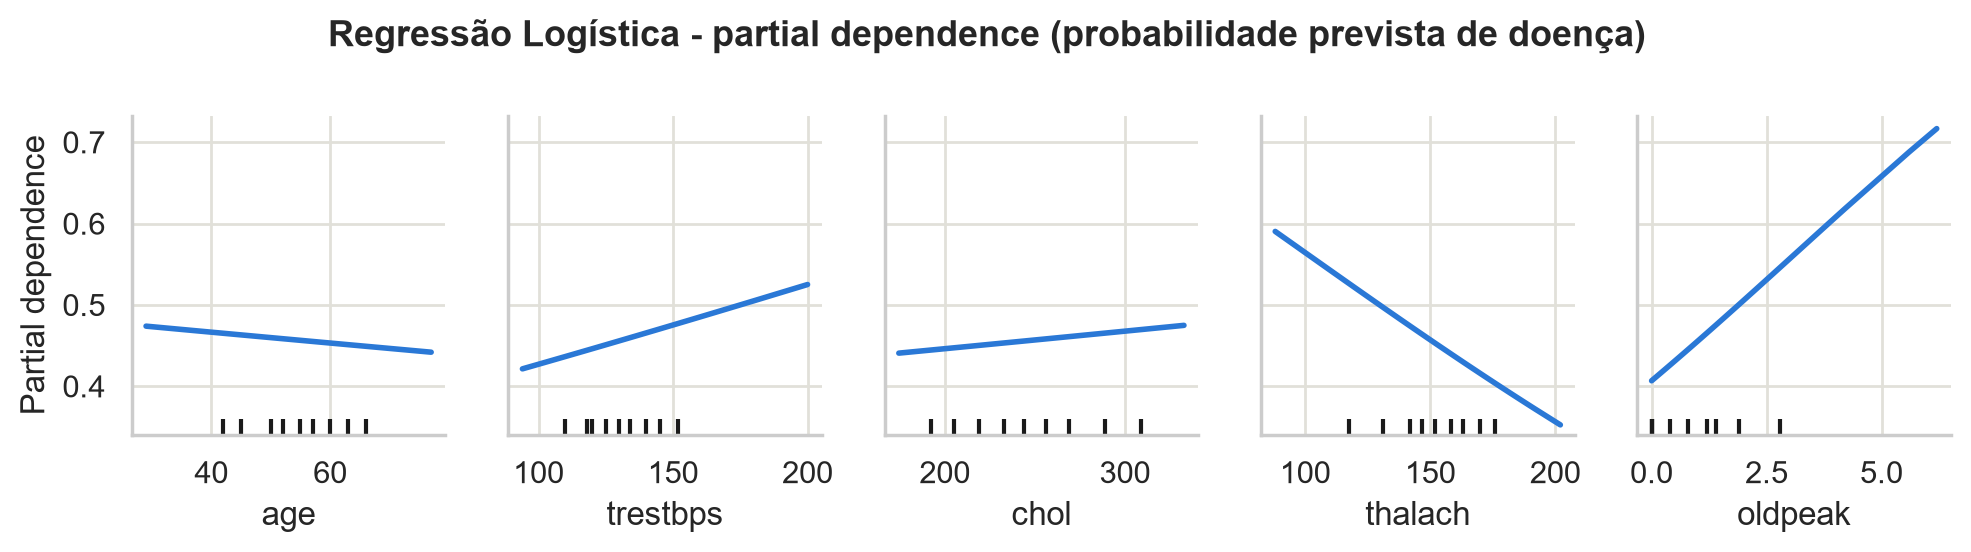
\includegraphics[width=\linewidth]{t2_pdp.png}
\legenda{Partial dependence: probabilidade média prevista de doença em função de cada atributo numérico.}
\end{figure}
\FloatBarrier
\begin{itemize}
\item \pendente{o modelo resolve a tarefa pelos motivos certos ou usa correlações espúrias?}
\item \pendente{alguma variável funciona como proxy de atributos sensíveis?}
\item \pendente{os padrões aprendidos fazem sentido para especialistas do domínio?}
\item \pendente{há diferenças nas features mais relevantes entre grupos?}
\end{itemize}

\secao{Ethical Considerations}
\begin{itemize}
\item \textbf{Dados sensíveis:} a base contém dados de saúde (exames e diagnóstico cardíaco) e o sexo dos pacientes; nomes e documentos foram substituídos por valores fictícios na base original da UCI. \pendente{como esses dados são tratados e protegidos}
\item \textbf{Impacto em vidas humanas:} \pendente{decisões que o modelo poderia informar e consequências de seus erros para os pacientes}
\item \textbf{Mitigações adotadas:} nenhuma restrição de fairness foi aplicada no treinamento; o desempenho foi avaliado por sexo, faixa etária e sua interseção, com IC 95\%. \pendente{outras mitigações}
\item \textbf{Riscos e potenciais danos:} \pendente{quem pode ser prejudicado, probabilidade e magnitude do dano}
\item \textbf{Casos de uso problemáticos:} \pendente{usos especialmente arriscados ou eticamente questionáveis}
\end{itemize}

\secao{Caveats and Recommendations}
\begin{itemize}
\item \pendente{limitações conhecidas não cobertas nas seções anteriores e grupos não representados nos dados de avaliação}
\item \pendente{testes adicionais antes de implantação, monitoramento, supervisão humana e gatilhos para retreinamento}
\item \pendente{características ideais de um dataset de avaliação e recomendações de uso responsável}
\end{itemize}

\vfill
{\footnotesize\textbf{Referências.}
BHAT, N. Health care: Data set on Heart attack possibility. Kaggle. \url{https://www.kaggle.com/datasets/nareshbhat/health-care-data-set-on-heart-attack-possibility}.
JANOSI, A.; STEINBRUNN, W.; PFISTERER, M.; DETRANO, R. Heart Disease [conjunto de dados]. UCI Machine Learning Repository, 1988. \url{https://doi.org/10.24432/C52P4X}.
MITCHELL, M. et al. Model Cards for Model Reporting. In: FAT* '19, 2019. \url{https://arxiv.org/abs/1810.03993}.\par}

\end{document}
